\documentclass[12pt]{article}
\usepackage[utf8]{inputenc}
\usepackage[T1]{fontenc}
\usepackage{fontspec}
\setmainfont{Times New Roman}
\newfontfamily\hackfont{Hack}
\usepackage{titlesec}
\usepackage{fancyhdr}
\usepackage{listings}
\usepackage{xcolor}
\usepackage{graphicx}
\usepackage{longtable}
\usepackage{caption}
\usepackage{hyperref}
\usepackage{setspace}
\usepackage{multirow}
\usepackage{array}
\usepackage{tikz}
\usepackage{geometry}
\geometry{a4paper, margin=1in}
\hypersetup{colorlinks=true, linkcolor=blue, urlcolor=blue}
\renewcommand{\contentsname}{Table of Contents}

\pagestyle{fancy}
\fancyhf{} 							% Header Middle
\rhead{Lab-07}
\lhead{Technical Writing}
\rfoot{\thepage}

\begin{document}

\begin{titlepage}					% Cover Start
\begin{center}
    
\includegraphics[width=0.35\textwidth]{logo.png} \\
    \vspace{0.5cm}
    \textbf{\Huge \textcolor{teal}{NOTRE DAME} \textcolor{teal}{UNIVERSITY}} \\
    \vspace{0.5cm}
    \textbf{\Huge \textcolor{orange}{BANGLADESH}} \\
    
    \vspace{0.9cm}
    \textbf{\Huge \underline{Technical Writing Lab Task-07}} \\
    
    \vspace{1.5em}
    \begin{flushleft}
    	\textbf{\Large Course Code: CSE-3207} \\
		\vspace{0.3cm}        
        \textbf{\Large Course Title: Technical Writing Presentation} \\
        \vspace{0.3cm}
        \textbf{\Large Lab Task Topic: Picture \& Table Formating in LaTaX} \\        
    \end{flushleft}
    
    \vspace{1em}
    \begin{flushleft}
        \textbf{\Huge \textcolor{blue}{Submitted by:}} \\
        \vspace{0.3cm}
        \textbf{\Large Name: Istiak Alam} \\
        \vspace{0.3cm}
        \textbf{\Large ID: 0692230005101005} \\
		\vspace{0.3cm}        
        \textbf{\Large Batch: CSE-20} \\
        \vspace{0.5cm}
        \textbf{\Large Submission Date: }{\Large \textbf{\today}\par}
    \end{flushleft}
    \vfill
    \begin{flushleft}
        \textbf{\Huge \textcolor{blue}{Submitted to:}} \\
        \vspace{0.3cm}
        \textbf{\Large Md. Tahmid Hasan} \\
        \vspace{0.3cm}
        \textbf{\Large Lecturer,} \\
        \vspace{0.3cm}
        \textbf{\Large Notre Dame University Bangladesh}
    \end{flushleft}
\end{center}
\end{titlepage}						% Cover End


\pagenumbering{arabic}

\section*{Question : Create this following Table in LaTeX}
\begin{figure}[h!]
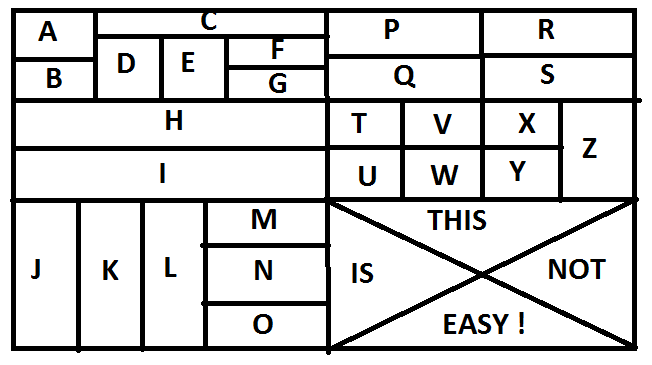
\includegraphics[width=1\textwidth]{table.png}
\caption{\label{table}Complex Table Sample output}
\end{figure}

\section*{Answer :}
\Large Let's Solve it from Table 1, 2, 3, 4
\subsection*{Table 1:}
\begin{center}
\setlength{\extrarowheight}{7pt}
\begin{tabular}{|c|c|c|c|}
\hline
A & \multicolumn{3}{c|}{C} \\
\hline
\multirow{2}{*}{B} & \multirow{2}{*}{D} & \multirow{2}{*}{E} & F \\
\cline{4-4}
 &  &  & G \\
\hline
\multicolumn{4}{|c|}{H} \\
\hline
\multicolumn{4}{|c|}{I} \\
\hline 
\end{tabular} 
\end{center}

\subsection*{Table 2:}
\begin{center}
\setlength{\extrarowheight}{10pt}
\begin{tabular}{|c|c|c|c|}
\hline
\multicolumn{2}{|c|}{P} & \multicolumn{2}{c|}{R} \\
\hline
\multicolumn{2}{|c|}{Q} & \multicolumn{2}{c|}{S} \\
\hline
T & V & X & \multirow{2}{*}{Z}\\
\cline{1-3}
U & W & Y &  \\
\hline
\end{tabular}
\end{center}

\subsection*{Table 3:}
\begin{center}
\setlength{\extrarowheight}{7pt}
\begin{tabular}{|c|c|c|c|}
\hline
\multirow{3}{*}{J} & \multirow{3}{*}{K} & \multirow{3}{*}{L} & M \\
\cline{4-4}
 &  &  & N \\
\cline{4-4}
 &  &  & O \\
\hline
\end{tabular}
\end{center}

\subsection*{Table 4:}
\begin{center}
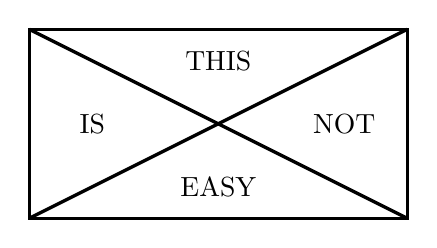
\begin{tikzpicture}[scale=0.8]
    % Draw the rectangle border
    \draw[very thick] (0,0) rectangle (6,3);

    % Draw diagonals
    \draw[very thick] (0,0) -- (6,3);
    \draw[very thick] (0,3) -- (6,0);

    % Add the text
    \node at (3,2.5) {THIS};
    \node at (1,1.5) {IS};
    \node at (5,1.5) {NOT};
    \node at (3,0.5) {EASY};
\end{tikzpicture}
\end{center}
\newpage

\section*{Combining All the 4 Tables:}
\begin{figure}[h!]
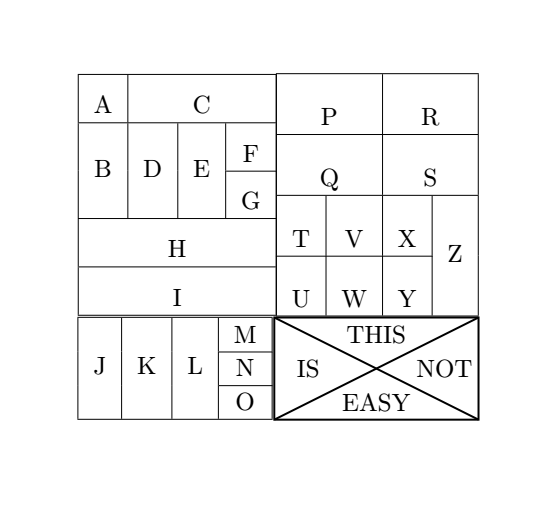
\includegraphics[width=1\textwidth]{ans.png}
\caption{\label{table}Complex table}
\end{figure}
\newpage
\section{Code in Texmaker:}
\begin{verbatim}
Table 1 : \\
\setlength{\extrarowheight}{7pt}
\begin{tabular}{|c|c|c|c|}
\hline
A & \multicolumn{3}{c|}{C} \\
\hline
\multirow{2}{*}{B} & \multirow{2}{*}{D} & 
\multirow{2}{*}{E} & F \\
\cline{4-4}
 &  &  & G \\
\hline
\multicolumn{4}{|c|}{H} \\
\hline
\multicolumn{4}{|c|}{I} \\
\hline 
\end{tabular} \\ \\

Table 2 : \\
\setlength{\extrarowheight}{10pt}
\begin{tabular}{|c|c|c|c|}
\hline
\multicolumn{2}{|c|}{P} & \multicolumn{2}{c|}{R} \\
\hline
\multicolumn{2}{|c|}{Q} & \multicolumn{2}{c|}{S} \\
\hline
T & V & X & \multirow{2}{*}{Z}\\
\cline{1-3}
U & W & Y &  \\
\hline
\end{tabular} \\ \\
Table 3 : \\
\setlength{\extrarowheight}{7pt}
\begin{tabular}{|c|c|c|c|}
\hline
\multirow{3}{*}{J} & \multirow{3}{*}{K} &
 \multirow{3}{*}{L} & M \\
\cline{4-4}
 &  &  & N \\
\cline{4-4}
 &  &  & O \\
\hline
\end{tabular} \\ \\

Table 4 : \\
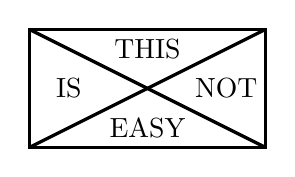
\begin{tikzpicture}[scale=0.5]
    % Draw the rectangle border
    \draw[very thick] (0,0) rectangle (6,3);

    % Draw diagonals
    \draw[very thick] (0,0) -- (6,3);
    \draw[very thick] (0,3) -- (6,0);

    % Add the text
    \node at (3,2.5) {THIS};
    \node at (1,1.5) {IS};
    \node at (5,1.5) {NOT};
    \node at (3,0.5) {EASY};
\end{tikzpicture} \\
\end{verbatim}

\newpage
\section*{Combined Code for 4 Tables:}
\begin{verbatim}
Combining 4 tables : \\

\setlength{\extrarowheight}{20pt}
\begin{tabular}{cc}

 \setlength{\extrarowheight}{7pt}
\begin{tabular}{|c|c|c|c|}
\hline
A & \multicolumn{3}{c|}{C} \\
\hline
\multirow{2}{*}{B} & \multirow{2}{*}{D} & 
\multirow{2}{*}{E} & F \\
\cline{4-4}
 &  &  & G \\
\hline
\multicolumn{4}{|c|}{H} \\
\hline
\multicolumn{4}{|c|}{I} \\
\hline 
\end{tabular}  &

\noindent
\makebox[0pt][l]{
\hspace{-0.9cm}

\setlength{\extrarowheight}{12pt}
\begin{tabular}{|c|c|c|c|}
\hline
\multicolumn{2}{|c|}{P} & \multicolumn{2}{c|}{R} \\
\hline
\multicolumn{2}{|c|}{Q} & \multicolumn{2}{c|}{S} \\
\hline
T & V & X & \multirow{2}{*}{Z}\\
\cline{1-3}
U & W & Y &  \\
\hline
\end{tabular} } \\

\raisebox{2.85cm}{
\makebox[0pt][l]{
\hspace{-1.7cm}

 \setlength{\extrarowheight}{1.5pt}
\begin{tabular}{|c|c|c|c|}
\hline
\multirow{3}{*}{J} & \multirow{3}{*}{K} & 
\multirow{3}{*}{L} & M \\
\cline{4-4}
 &  &  & N \\
\cline{4-4}
 &  &  & O \\
\hline
\end{tabular} } } & 

\raisebox{2.2cm}{
\makebox[0pt][l]{
\hspace{-0.82cm}
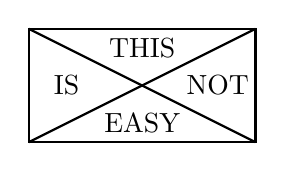
\begin{tikzpicture}[scale=0.48]
    % Here I use a rectangle border
    \draw[thick] (0,0) rectangle (6,3);


    % Here is a diagonals
    \draw[thick] (0,0) -- (6,3);
    \draw[thick] (0,3) -- (6,0);

    % using node for text
    \node at (3,2.5) {THIS};
    \node at (1,1.5) {IS};
    \node at (5,1.5) {NOT};
    \node at (3,0.5) {EASY};
\end{tikzpicture} } } \\

\end{tabular}
\end{verbatim}


\end{document}